\documentclass[a4paper,11pt]{article}

% Identificação
\newcommand{\pbtitulo}{Kafka}
\newcommand{\pbversao}{1.01}

\usepackage{../../sty/tutorial}

%----------------------------------------------------------------------
% Início do Documento
%----------------------------------------------------------------------
\begin{document}
	
	\maketitle % mostrar o título
	\thispagestyle{fancy} % habilitar o cabeçalho/rodapé das páginas
	
%--------------------------------------------------------------------------
% RESUMO DO ARTIGO
%--------------------------------------------------------------------------
\begin{abstract}
	% O primeiro caractere deve vir com \initial{}
	\initial{K}afka\cite{kafkaoficial} ou "Apache Kafka" (aqui chamarei apenas de Kafka) é parte do Ecosistema Hadoop e uma plataforma de streaming de eventos distribuída pela comunidade capaz de lidar com trilhões por dia. Inicialmente concebido como uma simples fila de mensagens, Kafka é baseado em uma abstração de um log de confirmação distribuído. Desde que foi criado e aberto pelo LinkedIn em 2011, evoluiu rapidamente da fila de mensagens para uma plataforma de streaming de eventos completa.
\end{abstract}

%--------------------------------------------------------------------------
% CONTEÚDO DO ARTIGO
%--------------------------------------------------------------------------
\section{Parte inicial}
Kafka é uma plataforma de streaming distribuída. Kafka pode ser usado para construir aplicativos de streaming em tempo real que podem transformar os fluxos de dados ou deduzir alguma inteligência deles. 

\begin{figure}[H]
	\centering
	
\includegraphics[width=0.4\textwidth]{imagem/logo}
	\caption{Logo do Apache Kafka}
\end{figure}

Kafka fornece um banco de dados de streaming de vários sistemas de origem. Kafka propõe ter os seguintes recursos mencionados para seus bancos de dados de streaming: \vspace{-1em}
\begin{itemize}
	\item Análise em tempo real de fluxos de \textit{Big Data}
	\item Carrega recursos tolerantes a falhas
	\item Sistema durável, escalável e rápido
	\item Permite o rastreamento de dados de IoT 
\end{itemize}

Kafka é integrado a pipelines de dados de streaming que compartilham dados entre sistemas e/ou aplicativos e também é integrado aos sistemas e aplicativos que consomem esses dados. Oferece suporte a uma variedade de casos de uso em que alta taxa de transferência e escalabilidade são vitais. Minimiza a necessidade de integrações ponto a ponto para compartilhamento de dados em determinados aplicativos, ele pode reduzir a latência para milissegundos. Isso significa que os dados estão disponíveis para os usuários mais rapidamente, o que pode ser vantajoso em casos de uso que exigem disponibilidade de dados em tempo real, como operações de TI e comércio eletrônico. 

\subsection{Como funcionam os bancos de dados de streaming?}
Quando um fluxo atinge um banco de dados de streaming em tempo real, é processado imediatamente. Esses dados podem ser usados por um aplicativo após sua análise.

As entradas de dados para um banco de dados de streaming são chamadas de "fluxos de dados". Esses fluxos de dados são eventos de sequências e são imutáveis. Os dados de entrada para um banco de dados são categorizados em duas camadas: \vspace{-1em}
\begin{itemize}
	\item A primeira é a streaming
	\item A segunda é criada pelo usuário com base no comportamento desses fluxos, que podem ser chamados de "Estatísticas de eventos". 
\end{itemize}
	
Essa análise de fluxo de entrada é armazenada em colunas e tabelas da mesma forma que é armazenada em um banco de dados relacional tradicional. A imagem a seguir apresenta o fluxograma para o funcionamento de um banco de dados de streaming: 
\begin{figure}[H]
	\centering
	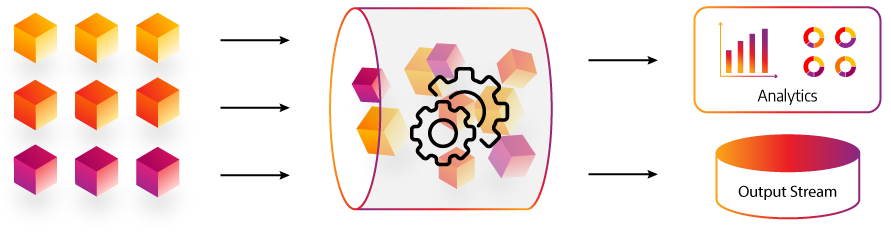
\includegraphics[width=0.8\textwidth]{imagem/BDStreaming}
	\caption{Representação do Banco de Dados de Streaming}
\end{figure}

Os dados reservados em um banco de dados de streaming podem ser informações do usuário de plataformas de mídia social, um arquivo de log gerado pela Web, tendências do usuário de comércio eletrônico, relatórios de atividade em um jogo ou telemetria de vários aplicativos em um \textit{data centers}. Esses dados são processados sequencialmente e incrementalmente e, em seguida, usados para fazer análises como regressão, filtragem, amostragem e correlação.

Essa análise de dados em tempo real abre vários casos de uso para diferentes setores. As empresas podem fazer uso dessa análise e tomar decisões relevantes com base nos resultados da análise. Considere um exemplo para uma organização, onde a análise de mídia social é feita por meio dos recursos de um banco de dados de streaming. A organização pode analisar facilmente o comportamento e a atividade do usuário. Essa observação pode ajudar a empresa a dar novos passos a partir dos dados analisados para melhorar a eficiência. 

\subsection{Criar a composição Docker}
A forma mais simples para obtermos o Kafka é através de um contêiner no Docker, deste modo podemos ter várias versões instalada e controlar mais facilmente qual está ativa ou não. E ainda colhemos o benefício adicional de não termos absolutamente nada deixando sujeira em nosso sistema operacional ou áreas de memória.

Precisamos do Zookeeper para termos o Kafka. Qual o papel do Zookeeper? É usado para selecionar automaticamente um líder para uma partição. Em caso de desligamento de algum broker, é realizada uma reeleição, pelo ZooKeeper, para a posição de líder das partições (que caíram com o broker). Também metadados como, em qual corretor uma partição líder está vivendo. Esses detalhes são mantidos pelo ZooKeeper. Produtores que transmitem dados para tópicos ou Consumidores que leem os dados do fluxo de tópicos entrem em contato com o ZooKeeper para obter o broker mais próximo ou menos ocupado. 

Se olhou a apostila do Zookeeper (caso não recomendo) criamos uma composição de 3 servidores com o Docker Compose, esse é usado exatamente quando precisamos simular várias máquinas. Assim vamos adicionar o Kafka a esta composição. Editar o arquivo docker-compose.yml: \\
\codigo{\$ vim docker-compose.yml}

E o deixamos com a seguinte codificação:
\begin{lstlisting}[]
version: '3.1'

services:
  zoo1:
    image: zookeeper
    container_name: meu-zoo1
    init: true
    restart: always
    hostname: zoo1
    ports:
      - 2181:2181
      - 8081:8080
    environment:
      ZOO_MY_ID: 1
      ZOO_SERVERS: server.1=zoo1:2888:3888;2181 server.2=zoo2:2888:3888;2181 server.3=zoo3:2888:3888;2181

  zoo2:
    image: zookeeper
    container_name: meu-zoo2
    restart: always
    init: true
    hostname: zoo2
    ports:
      - 2182:2181
      - 8082:8080 
    environment:
      ZOO_MY_ID: 2
      ZOO_SERVERS: server.1=zoo1:2888:3888;2181 server.2=zoo2:2888:3888;2181 server.3=zoo3:2888:3888;2181

  zoo3:
    image: zookeeper
    container_name: meu-zoo3
    restart: always
    init: true
    hostname: zoo3
    ports:
      - 2183:2181
      - 8083:8080
    environment:
      ZOO_MY_ID: 3
      ZOO_SERVERS: server.1=zoo1:2888:3888;2181 server.2=zoo2:2888:3888;2181 server.3=zoo3:2888:3888;2181
      
  kafka:
    image: confluentinc/cp-kafka:latest
    container_name: meu-kafka
    depends_on:
      - zoo1
      - zoo2
      - zoo3
    ports:
      - 9092:9092
    environment:
      KAFKA_ZOOKEEPER_CONNECT: zoo1:2181,zoo2:2181,zoo3:2181
      KAFKA_ADVERTISED_LISTENERS: PLAINTEXT://localhost:9092
      KAFKA_OFFSETS_TOPIC_REPLICATION_FACTOR: 1
\end{lstlisting}
	
Salvamos o arquivo com ESC e o comando \textbf{:wq}, agora vem a parte divertida, usamos o comando: \\
\codigo{\$ docker-compose down}

Caso já exista os contêineres do Zookeeper criados, e iniciamos novamente a composição com: \\
\codigo{\$ docker-compose up -d}

A \textbf{Confluent}\cite{confluentoficial} é uma empresa fundada pelos desenvolvedores do Kafka. Fornecem conectores adicionais ao Kafka por meio de versões Aberta e Comercial do Confluent Kafka. Também oferecem suporte por meio de qualquer Kafka Cluster ou configuração de aplicativo, caso necessite em sua organização.

\section{Compreender o uso da composição Docker}
Docker Compose é usado quando temos vários contêineres que dependem uns dos outros e precisamos mantê-los juntos, isso significa subir ou parar em uma ordem determinada, questões de dependências ou acessos.

Automaticamente para essa composição é criada uma rede Docker que os mantêm no mesmo servidor com portas diferentes. Por exemplo, nesta temos 3 Zookeeper e 1 Kafka, cada um possui uma porta determinada, acessando a página: \\
\url{http://localhost:8081/commands/}

Acessamos o primeiro Zookeeper (contêiner meu-zoo1), os outros estão na porta 8082 e 8083 respectivamente, acesse agora a opção \textbf{leader}. Isso identifica qual o servidor líder, vamos supor que seja o 3 (essa eleição é feita aleatoriamente), acesse a seguinte página: \\
\url{http://localhost:8083/commands/connections}

E veremos nesta a conexão do Kafka.
\begin{figure}[H]
	\centering
	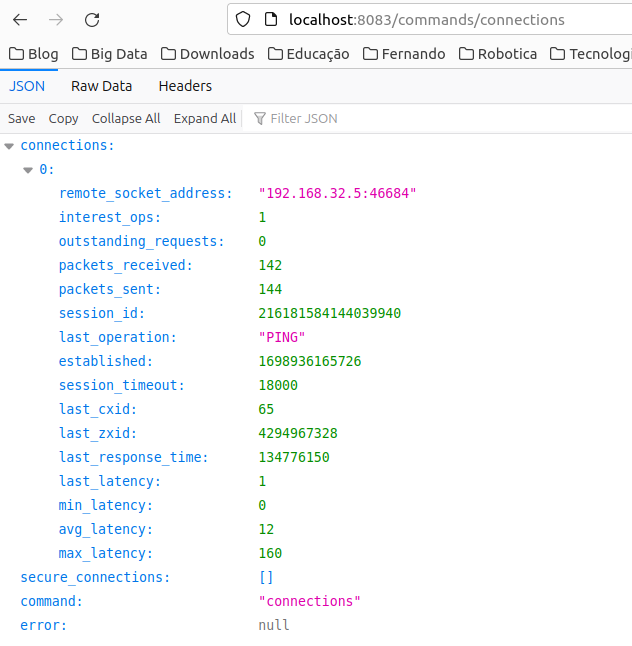
\includegraphics[width=0.6\textwidth]{imagem/conexaozoo}
	\caption{Kafka conectado ao Zookeeper}
\end{figure}

Vamos dar prosseguimento e veremos como performam as mensagens.

\section{Produzir e Consumir mensagens}
Vamos usar o \textbf{NodeJS} para exemplificar como podemos verificar o funcionamento do serviço Kafka. O primeiro passo é criar uma pasta e inicializá-la com o NodeJS: \\
\codigo{\$ npm init -y}

Precisamos também da biblioteca de comunicação com o Kafka: \\
\codigo{\$ npm install kafkajs}

O \textbf{tópico} é uma categoria na qual os fluxos de eventos/registros são armazenados no cluster Kafka. Um cluster Kafka pode ter vários tópicos. Criamos um programa chamado "topic.js" com o seguinte conteúdo:
\begin{lstlisting}[]
const { Kafka } = require("kafkajs");

run();

async function run() {
  try {
    const kafka = new Kafka({
      "clientId": "myapp",
      "brokers": ["localhost:9092"]
    });
    const admin = kafka.admin();
    console.log("Conectando...");
    await admin.connect();
    console.log("Conectado!");
    await admin.createTopics({
      "topics": [{
        "topic": "Usuarios",
        "numPartitions": 2
      }]
    });
    console.log("Sucesso");
    await admin.disconnect();
    console.log("Desconectado!");
  } catch (ex) {
    console.error(`Alguma coisa aconteceu ${ex}`)
  } finally {
    process.exit(0);
  }
}
\end{lstlisting}

E rodamos este com o seguinte comando: \\
\codigo{\$ node topic.js}

Se olharmos no "log" deste contêiner: \\
\codigo{\$ docker logs meu-kafka}

Veremos que foi criado um tópico chamado "Usuarios" com duas partições. Iniciando com:  \vspace{-1em}
\begin{verbatim}
INFO Created log for partition Usuarios-0 in /var/lib/kafka/data/Usuarios-0 with
 properties {} (kafka.log.LogManager)
\end{verbatim} \vspace{-1em}

Podemos, em seguida, criar nosso produtor de conteúdo. Produtores são aplicativos que enviam fluxos de dados para tópicos no Kafka Cluster. Um produtor pode enviar o fluxo de registros para vários tópicos. A API do Apache Kafka Producer permite que um aplicativo se torne um produtor. Criamos um programa chamado "producer.js" com o seguinte conteúdo:
\begin{lstlisting}[]
const { Kafka } = require("kafkajs");
const usuario = process.argv[2];

run();

async function run() {
  try {
    const kafka = new Kafka({
      "clientId": "myapp",
      "brokers": ["ip:9092"]
    });
    const producer = kafka.producer();
    console.log("Conectando...");
    await producer.connect();
    console.log("Produtor Conectado!");

    // A-M = Part0 ou N-Z = Part1
    const particao = usuario[0] < "N" ? 0 : 1;

    const result = await producer.send({
      "topic": "Usuarios",
      "messages": [
        {
          "value": usuario,
          "partition": particao
        }
      ]
    });
    console.log(`Mensagem Enviada: ${JSON.stringify(result)}`);
    await producer.disconnect();
    console.log("Produtor Desconectado!");
  } catch (ex) {
    console.error(`Alguma coisa aconteceu ${ex}`)
  } finally {
    process.exit(0);
  }
}
\end{lstlisting}

E rodamos este com o seguinte comando: \\
\codigo{\$ node producer.js nomequalquer}

Para este exemplo insira um nome não composto (para isso devemos usar as aspas, e o programa não está preparado), pois a primeira letra da palavra vai definir em qual partição esse usuário vai entrar entre as letras "A" e "M" será a partição 0 e de "N" a "Z" na 1. Rodamos esse comando algumas vezes adicionando nomes de usuários para a nossa lista e vamos finalmente tratar do consumidor. 

Os consumidores são aplicativos que se alimentam de fluxos de dados de tópicos no Kafka Cluster. Um consumidor pode receber fluxo de registros de vários tópicos por meio de assinatura. A API de consumidor do Apache Kafka permite que um aplicativo se torne um consumidor. Criamos um programa chamado "consumer.js" com o seguinte conteúdo:
\begin{lstlisting}[]
const { Kafka } = require("kafkajs");

run();

async function run() {
  try {
    const kafka = new Kafka({
      "clientId": "myapp",
      "brokers": ["192.168.15.5:9092"]
    });
    const consumer = kafka.consumer({ "groupId": "teste" });
    console.log("Conectando...");
    await consumer.connect();
    console.log("Consumidor Conectado!");
    consumer.subscribe({
      "topic": "Usuarios",
      "fromBeginning": true
    })

    await consumer.run({
      "eachMessage": async result => {
        console.log(`Mensagem recebida ${result.message.value} da partição ${result.partition}`);
      }
    });
    console.log("Consumidor Rodando...");
  } catch (ex) {
    console.error(`Alguma coisa aconteceu ${ex}`)
  }
}
\end{lstlisting}

Devemos observar que o comando "process.exit(0)" foi removido, assim como o comando para "desconectar", pois o consumidor deve ficar sempre rodando e recebendo as mensagens enviadas pelo produtor. Caso precise interrompê-lo usar o comando CRTL+C.

E rodamos este com o seguinte comando: \\
\codigo{\$ node consumer.js}

Todas as mensagens caem para esse consumidor, se abrirmos uma janela e executamos o produtor veremos que pouco importa se usamos a partição 0 ou 1 as mensagens caem para esse consumidor. Como mudar essa situação? simples abrimos mais uma janela e iniciamos um segundo consumidor. Agora o primeiro recebe mensagens somente da partição 0 enquanto que o segundo da 1.

\section{Interrupções no Zookeeper}
Agora que temos um ambiente de simulação com 3 Zookeeper e 2 consumidores do Kafka podemos simular o que acontece se a máquina que contém servidor do Zookeeper cair. Para isso vamos parar o contêiner (sabemos que o eleito foi o meu-zoo3): \\
\codigo{\$ docker stop meu-zoo3}

E com o produtor enviamos mais um usuário: \\
\codigo{\$ node producer.js NomeUsuario}

Observe que nos consumidores as mensagens continuam caindo sem o menor problema, como se nada tivesse ocorrido. Veja que realmente o servidor meu-zoo3 está fora do ar: \\
\url{http://localhost:8083/commands/connections}

Verificamos as conexões dos outros servidores: \\
\url{http://localhost:8081/commands/connections} e \\ 
\url{http://localhost:8082/commands/connections}

E verificamos que um dos dois assumiu essa conexão e manteve todo o fluxo em funcionamento. Podemos ativar novamente o contêiner: \\
\codigo{\$ docker start meu-zoo3}

Mas mesmo assim a conexão permanece no servidor eleito.

\section{Sistema em Java}
Nada disso teria graça senão usássemos Java para demonstrar o poder do Kafka, para isso vamos utilizar o Spring Tool Suite no qual criamos um projeto \textit{Maven Project}.

A grande vantagem de criarmos um projeto tipo Maven que podemos inserir todas as bibliotecas que necessitamos sem termos o menor trabalho, basta apenas buscamos estas do repositório central do Maven através de sua declaração no arquivo \textbf{pom.xml}:
\begin{lstlisting}[]
<project xmlns="http://maven.apache.org/POM/4.0.0"
 xmlns:xsi="http://www.w3.org/2001/XMLSchema-instance"
 xsi:schemaLocation="http://maven.apache.org/POM/4.0.0 https://maven.apache.org/xsd/maven-4.0.0.xsd">
  <modelVersion>4.0.0</modelVersion>
  <groupId>kafkaproj</groupId>
  <artifactId>kafkaproj</artifactId>
  <version>0.0.1-SNAPSHOT</version>
  <name>Projeto em Kafka</name>
  <description>Exemplo do projeto em Kafka</description>
  <dependencies>
    <dependency>
      <groupId>org.apache.kafka</groupId>
      <artifactId>kafka_2.13</artifactId>
      <version>3.1.0</version>
    </dependency>
    <dependency>
      <groupId>org.apache.kafka</groupId>
      <artifactId>kafka-clients</artifactId>
      <version>3.1.0</version>
    </dependency>
    <dependency>
      <groupId>com.typesafe.scala-logging</groupId>
      <artifactId>scala-logging-slf4j_2.11</artifactId>
      <version>2.1.2</version>
    </dependency>
  </dependencies>
</project>
\end{lstlisting}

Assim de forma simples temos as bibliotecas do Kafka e do Log do Scala que é utilizada pela classe \textit{ShutdownableThread} que usaremos para manter o consumidor ativo. Vamos começar com a classe que produz nossas mensagens, criamos uma classe chamada \textbf{ExProdutor} com a seguinte codificação:
\begin{lstlisting}[]
package kafkaproj;

import java.util.Properties;
import java.util.concurrent.ExecutionException;

import org.apache.kafka.clients.producer.Callback;
import org.apache.kafka.clients.producer.KafkaProducer;
import org.apache.kafka.clients.producer.ProducerRecord;
import org.apache.kafka.clients.producer.RecordMetadata;
 
public class ExProdutor extends Thread {
  private final KafkaProducer<Integer, String> producer;
  private final String topic;
  private final boolean isAsync;
 
  public static final String KAFKA_SERVER_URL = "localhost";
  public static final int KAFKA_SERVER_PORT = 9092;
  public static final String CLIENT_ID = "SimplesProdutor";
 
  public ExProdutor(String topic, Boolean isAsync) {
    Properties properties = new Properties();
    properties.put("bootstrap.servers", KAFKA_SERVER_URL + ":" + KAFKA_SERVER_PORT);
    properties.put("client.id", CLIENT_ID);
    properties.put("key.serializer", "org.apache.kafka.common.serialization.IntegerSerializer");
    properties.put("value.serializer", "org.apache.kafka.common.serialization.StringSerializer");
    producer = new KafkaProducer<>(properties);
    this.topic = topic;
    this.isAsync = isAsync;
  }
 
  @Override
  public void run() {
    for (int messageNo = 1; messageNo < 100; messageNo++) {
      String messageStr = "Esta é a mensagem no." + messageNo;
      long startTime = System.currentTimeMillis();
      if (isAsync) {
        producer.send(new ProducerRecord<>(topic, messageNo,
          messageStr), new DemoCallBack(startTime, messageNo, messageStr));
      } else {
        try {
          producer.send(new ProducerRecord<>(topic, messageNo, messageStr)).get();
          System.out.println("Enviando mensagem: (" + messageNo + ", " + messageStr + ")");
        } catch (InterruptedException e) {
          e.printStackTrace();
          Thread.currentThread().interrupt();
        } catch (ExecutionException e) {
          e.printStackTrace();
        }
      }
    }
  }
}
 
class DemoCallBack implements Callback {
 
  private final long startTime;
  private final int key;
  private final String message;
 
  public DemoCallBack(long startTime, int key, String message) {
    this.startTime = startTime;
    this.key = key;
    this.message = message;
  }
 
  public void onCompletion(RecordMetadata metadata, Exception exception) {
    long elapsedTime = System.currentTimeMillis() - startTime;
    if (metadata != null) {
      System.out.println(
        "message(" + key + ", " + message + ") sent to partition(" + metadata.partition() + "), " +
                 "offset(" + metadata.offset() + ") in " + elapsedTime + " ms");
    } else {
      exception.printStackTrace();
    }
  }
}
\end{lstlisting}

Para executá-la uma simples classe que contém o método main() chamada \textbf{GeraMensagens}:
\begin{lstlisting}[]
package kafkaproj;

public class GeraMensagens {
  public static final String TOPIC = "testTopic";
   
  public static void main(String[] args) {
    boolean isAsync = false;
    ExProdutor producerThread = new ExProdutor(TOPIC, isAsync);
    producerThread.start();
  }
}
\end{lstlisting}

Para consumirmos as mensagens geradas, criamos uma classe chamada \textbf{ExConsumidor} com a seguinte codificação:
\begin{lstlisting}[]
package kafkaproj;

import java.time.Duration;
import java.util.Collections;
import java.util.Properties;

import org.apache.kafka.clients.consumer.ConsumerConfig;
import org.apache.kafka.clients.consumer.ConsumerRecord;
import org.apache.kafka.clients.consumer.ConsumerRecords;
import org.apache.kafka.clients.consumer.KafkaConsumer;

import kafka.utils.ShutdownableThread;

public class ExConsumidor extends ShutdownableThread {
  private final KafkaConsumer<Integer, String> consumer;
  private final String topic;
     
  public static final String KAFKA_SERVER_URL = "localhost";
  public static final int KAFKA_SERVER_PORT = 9092;
  public static final String CLIENT_ID = "SimplesConsumidor";
 
  public ExConsumidor(String topic) {
    super("KafkaConsumidor", false);
    Properties props = new Properties();
    props.put(ConsumerConfig.BOOTSTRAP_SERVERS_CONFIG, KAFKA_SERVER_URL + ":" + KAFKA_SERVER_PORT);
    props.put(ConsumerConfig.GROUP_ID_CONFIG, CLIENT_ID);
    props.put(ConsumerConfig.ENABLE_AUTO_COMMIT_CONFIG, "true");
    props.put(ConsumerConfig.AUTO_COMMIT_INTERVAL_MS_CONFIG, "1000");
    props.put(ConsumerConfig.SESSION_TIMEOUT_MS_CONFIG, "30000");
    props.put(ConsumerConfig.KEY_DESERIALIZER_CLASS_CONFIG, "org.apache.kafka.common.serialization.IntegerDeserializer");
    props.put(ConsumerConfig.VALUE_DESERIALIZER_CLASS_CONFIG, "org.apache.kafka.common.serialization.StringDeserializer");
 
    consumer = new KafkaConsumer<>(props);
    this.topic = topic;
  }
 
  @Override
  public void doWork() {
    consumer.subscribe(Collections.singletonList(this.topic));
    ConsumerRecords<Integer, String> records = consumer.poll(Duration.ofMillis(100));
    for (ConsumerRecord<Integer, String> registro : records) {
      System.out.println("Recebendo mensagem: (" + registro.key() + ", " + registro.value() + ") at offset " + registro.offset());
    }
  }
 
  @Override
  public String name() {
    return null;
  }
 
  @Override
  public boolean isInterruptible() {
    return false;
  }
}
\end{lstlisting}

E finalmente para executá-la uma simples classe que contém o método main() chamada \textbf{ConsumeMensagens}:
\begin{lstlisting}[]
package kafkaproj;

public class ConsumeMensagens {
  public static void main(String[] args) {
    ExConsumidor consumerThread = new ExConsumidor("testTopic");
    consumerThread.start();
  }
}
\end{lstlisting}

Cada vez são geradas 100 mensagens para o "testTopic", o padrão de mensagem pode ser qualquer coisa que desejamos, o que mais impressiona nesse sistema é a velocidade como essas mensagens são consumidas de forma quase instantânea. Não pense que é porquê estamos na mesma máquina, Kafka foi criado para ser um sistema extremamente performático. 

Imagine então que através dele sistemas totalmente heterogêneos e que antes não trocavam informações agora podem fazê-lo sem o menor problema. E em linguagens totalmente diferentes. 

\section{Encerrando a composição}
Encerramos nossa composição com: \\
\codigo{\$ docker-compose stop}

Ou iniciarmos com: \\
\codigo{\$ docker-compose start}

Mas sempre na pasta que se encontra o arquivo \textbf{docker-compose.yml}. Mais fontes de informação podem ser obtidas em diversos sites que apresenta tutoriais completos sobre Kafka como a Tutorials Point\cite{tutorialspoint}.
	
\section{Conclusão}
Kafka é ideal para justificar a necessidade que o mundo tem gerado um volume cada vez maior de informações. Um cenário comum é que estes dados, uma vez gerados, precisam ser transportados para diversas aplicações. Kafka é uma plataforma de streaming de dados distribuído que pode publicar, assinar, armazenar e processar streams de registros em tempo real. Projetado para lidar com fluxos de dados de várias fontes e entregá-los a vários consumidores. Em resumo: mover grandes quantidades de dados – não apenas do ponto A ao B, mas dos pontos A ao Z e a qualquer outro lugar que necessitemos e tudo ao mesmo tempo.

E uma alternativa natural a um sistema de mensagens corporativo tradicional. Começou como um simples sistema interno desenvolvido pelo Linkedin para lidar com 1,4 trilhão de mensagens por dia, mas agora é uma solução de streaming de dados de código aberto com aplicação para uma variedade de necessidades corporativas. 

Kafka pode lidar com milhões de dados por segundo, o que o torna adequado para desafios de Big Data. No entanto, Kafka também faz sentido para empresas que atualmente não estão lidando com cenários de dados tão extremos. Em muitos casos de uso de processamento de dados, como Internet das Coisas (IoT) e mídia social, os dados estão aumentando exponencialmente e podem sobrecarregar rapidamente um aplicativo que estamos criando com base no volume de dados atual. Em termos de processamento de dados, podemos considerar a escalabilidade, e isso significa planejar a maior proliferação dos dados. 

Sou um entusiasta do mundo \textbf{Open Source} e novas tecnologias. Qual a diferença entre Livre e Open Source? \underline{Livre} significa que esta apostila é gratuita e pode ser compartilhada a vontade. \underline{Open Source} além de livre todos os arquivos que permitem a geração desta (chamados de arquivos fontes) devem ser disponibilizados para que qualquer pessoa possa modificar ao seu prazer, gerar novas, complementar ou fazer o que quiser. Os fontes da apostila (que foi produzida com o LaTex) está disponibilizado no GitHub \cite{github}. Veja ainda outros artigos que publico sobre tecnologia através do meu Blog Oficial \cite{fernandoanselmo}.

%--------------------------------------------------------------------------
% REFERÊNCIAS
%--------------------------------------------------------------------------
\begin{thebibliography}{4}
	\bibitem{kafkaoficial} 
	Página do Apache Kafka \\
	\url{https://kafka.apache.org/}

	\bibitem{confluentoficial} 
	Página da Confluent \\
	\url{https://www.confluent.io/what-is-apache-kafka/}
	
	\bibitem{tutorialspoint} 
	Tutorials Point sobre Kafka \\
	\url{https://www.tutorialspoint.com/apache_kafka/index.htm}	
	
		\bibitem{fernandoanselmo} 
	Fernando Anselmo - Blog Oficial de Tecnologia \\
	\url{http://www.fernandoanselmo.blogspot.com.br/}
	
	\bibitem{publicacao} 
	Encontre essa e outras publicações em \\
	\url{https://cetrex.academia.edu/FernandoAnselmo}
	
	\bibitem{github} 
	Repositório para os fontes da apostila \\
	\url{https://github.com/fernandoans/publicacoes}
\end{thebibliography}

\end{document}